\documentclass[12pt]{article}
\usepackage{graphicx}
\title{User Guide: HDMI output peripheral}
\author{Ana Klimovic, Bryce Long, Victor Zhang}


\begin{document}
  \maketitle
  Version for EDK 14.2
  \section{Goals}
  Use a custom HDMI output peripheral that displays a frame from off-chip memory.
  \section{Examples}
  You have been given two example projects that use the HDMI output peripheral. The first example uses a resolution of 640x480 and uses RGB565. The second example uses a resolution of 1280x720 and uses RGB888x. The peripheral supports 3 resolutions (640x480, 800x600, and 1280x720) and two colour formats (RGB565 and RGB888x).
  \section{Setup}
  \begin{enumerate}
    \item Start XPS and select \textbf {Open Project}. Browse to the \textbf {system.xmp} file in \textbf {ip\textbackslash{}hdmi\_out} and open the project. The BSB package is already selected for the \textit {Atlys} board.
    \item Click on \textbf {Generate Bitstream} and wait for the design to compile. This will take a few minutes.
    \item Click on \textbf {Export Design} and select to launch Xilinx Software Development Kit. Use the workspace in \textbf {ip\textbackslash{}workspace}.
    \item Create a new Xilinx C Project and select Empty Application. Also create a new BSP project.
    \item Copy the source files from \textbf {ip\textbackslash{}workspace\textbackslash{}hdmi\_out\_test\textbackslash{}src} including \textbf {lscript.ld}, the linker file, into your Xilinx C Project.
    \item Compile the project and Program the FPGA using the \textit {.elf} file you just compiled.
    \item If you have the UART connected, you should see \texttt {passed} being printed. This checks that the off-chip memory is connected properly. On the monitor, you should see an animation of a colourful gradient, slowly being covered with white pixels. This animation cycles continuously.
      \begin{figure}[h!]
        \centering
        \fbox{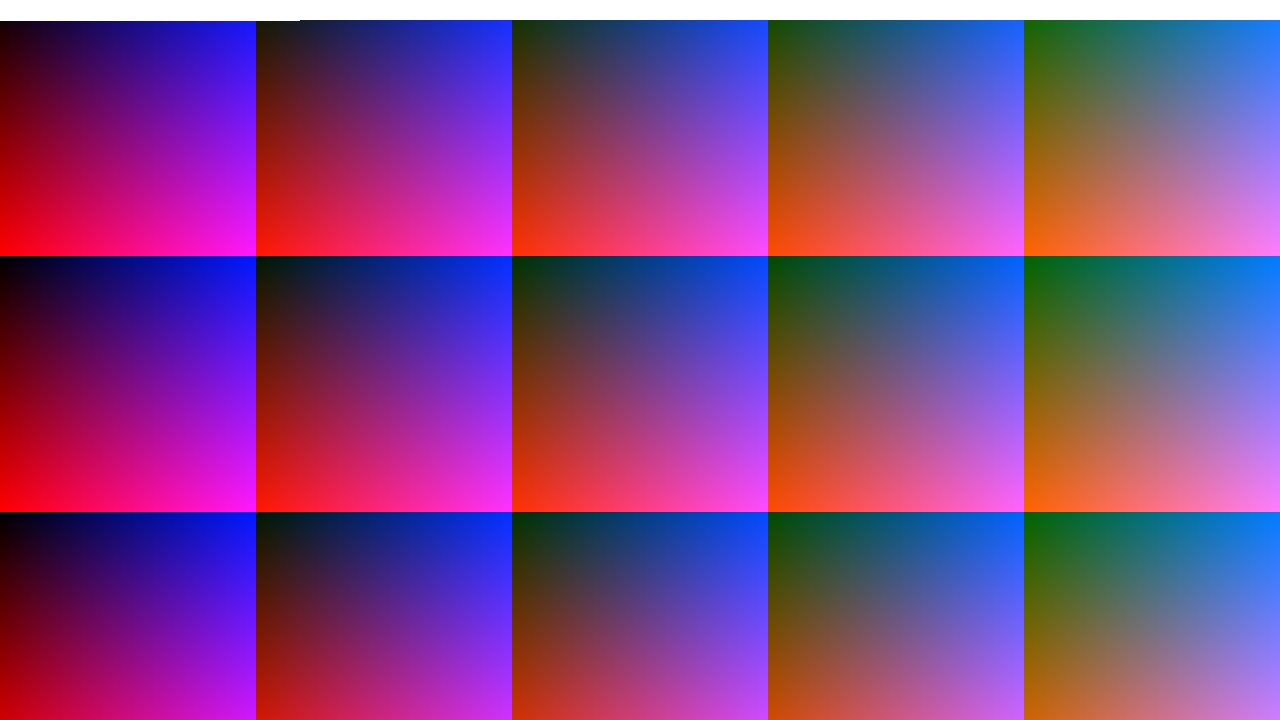
\includegraphics[width=6in]{ref1.jpg}}
        \caption{The start of the correct animation (1280x720, RGB888x)}
      \end{figure}
      \newpage
      \begin{figure}[h!]
        \centering
        \fbox{
\includegraphics[width=6in]{ref2.jpg}}
        \caption{Later on in the animation (1280x720, RGB888x)}
      \end{figure}
  \end{enumerate}
  \section{Block Diagram}
  This sections presents several block diagrams to illustrate how the HDMI output peripheral
  works. Figure 2 shows the system architecture involving the MicroBlaze,
  memory, the AXI bus interconnect, the screen and how they interact with the HDMI out IP.
  Figure 4 zooms in on the HDMI IP itself, showing the main blocks the IP is
  composed of. Finally, Figure 5 shows the detailed implementation of the
  user logic that forms the IP.
	\begin{figure}
	\centering
	\fbox{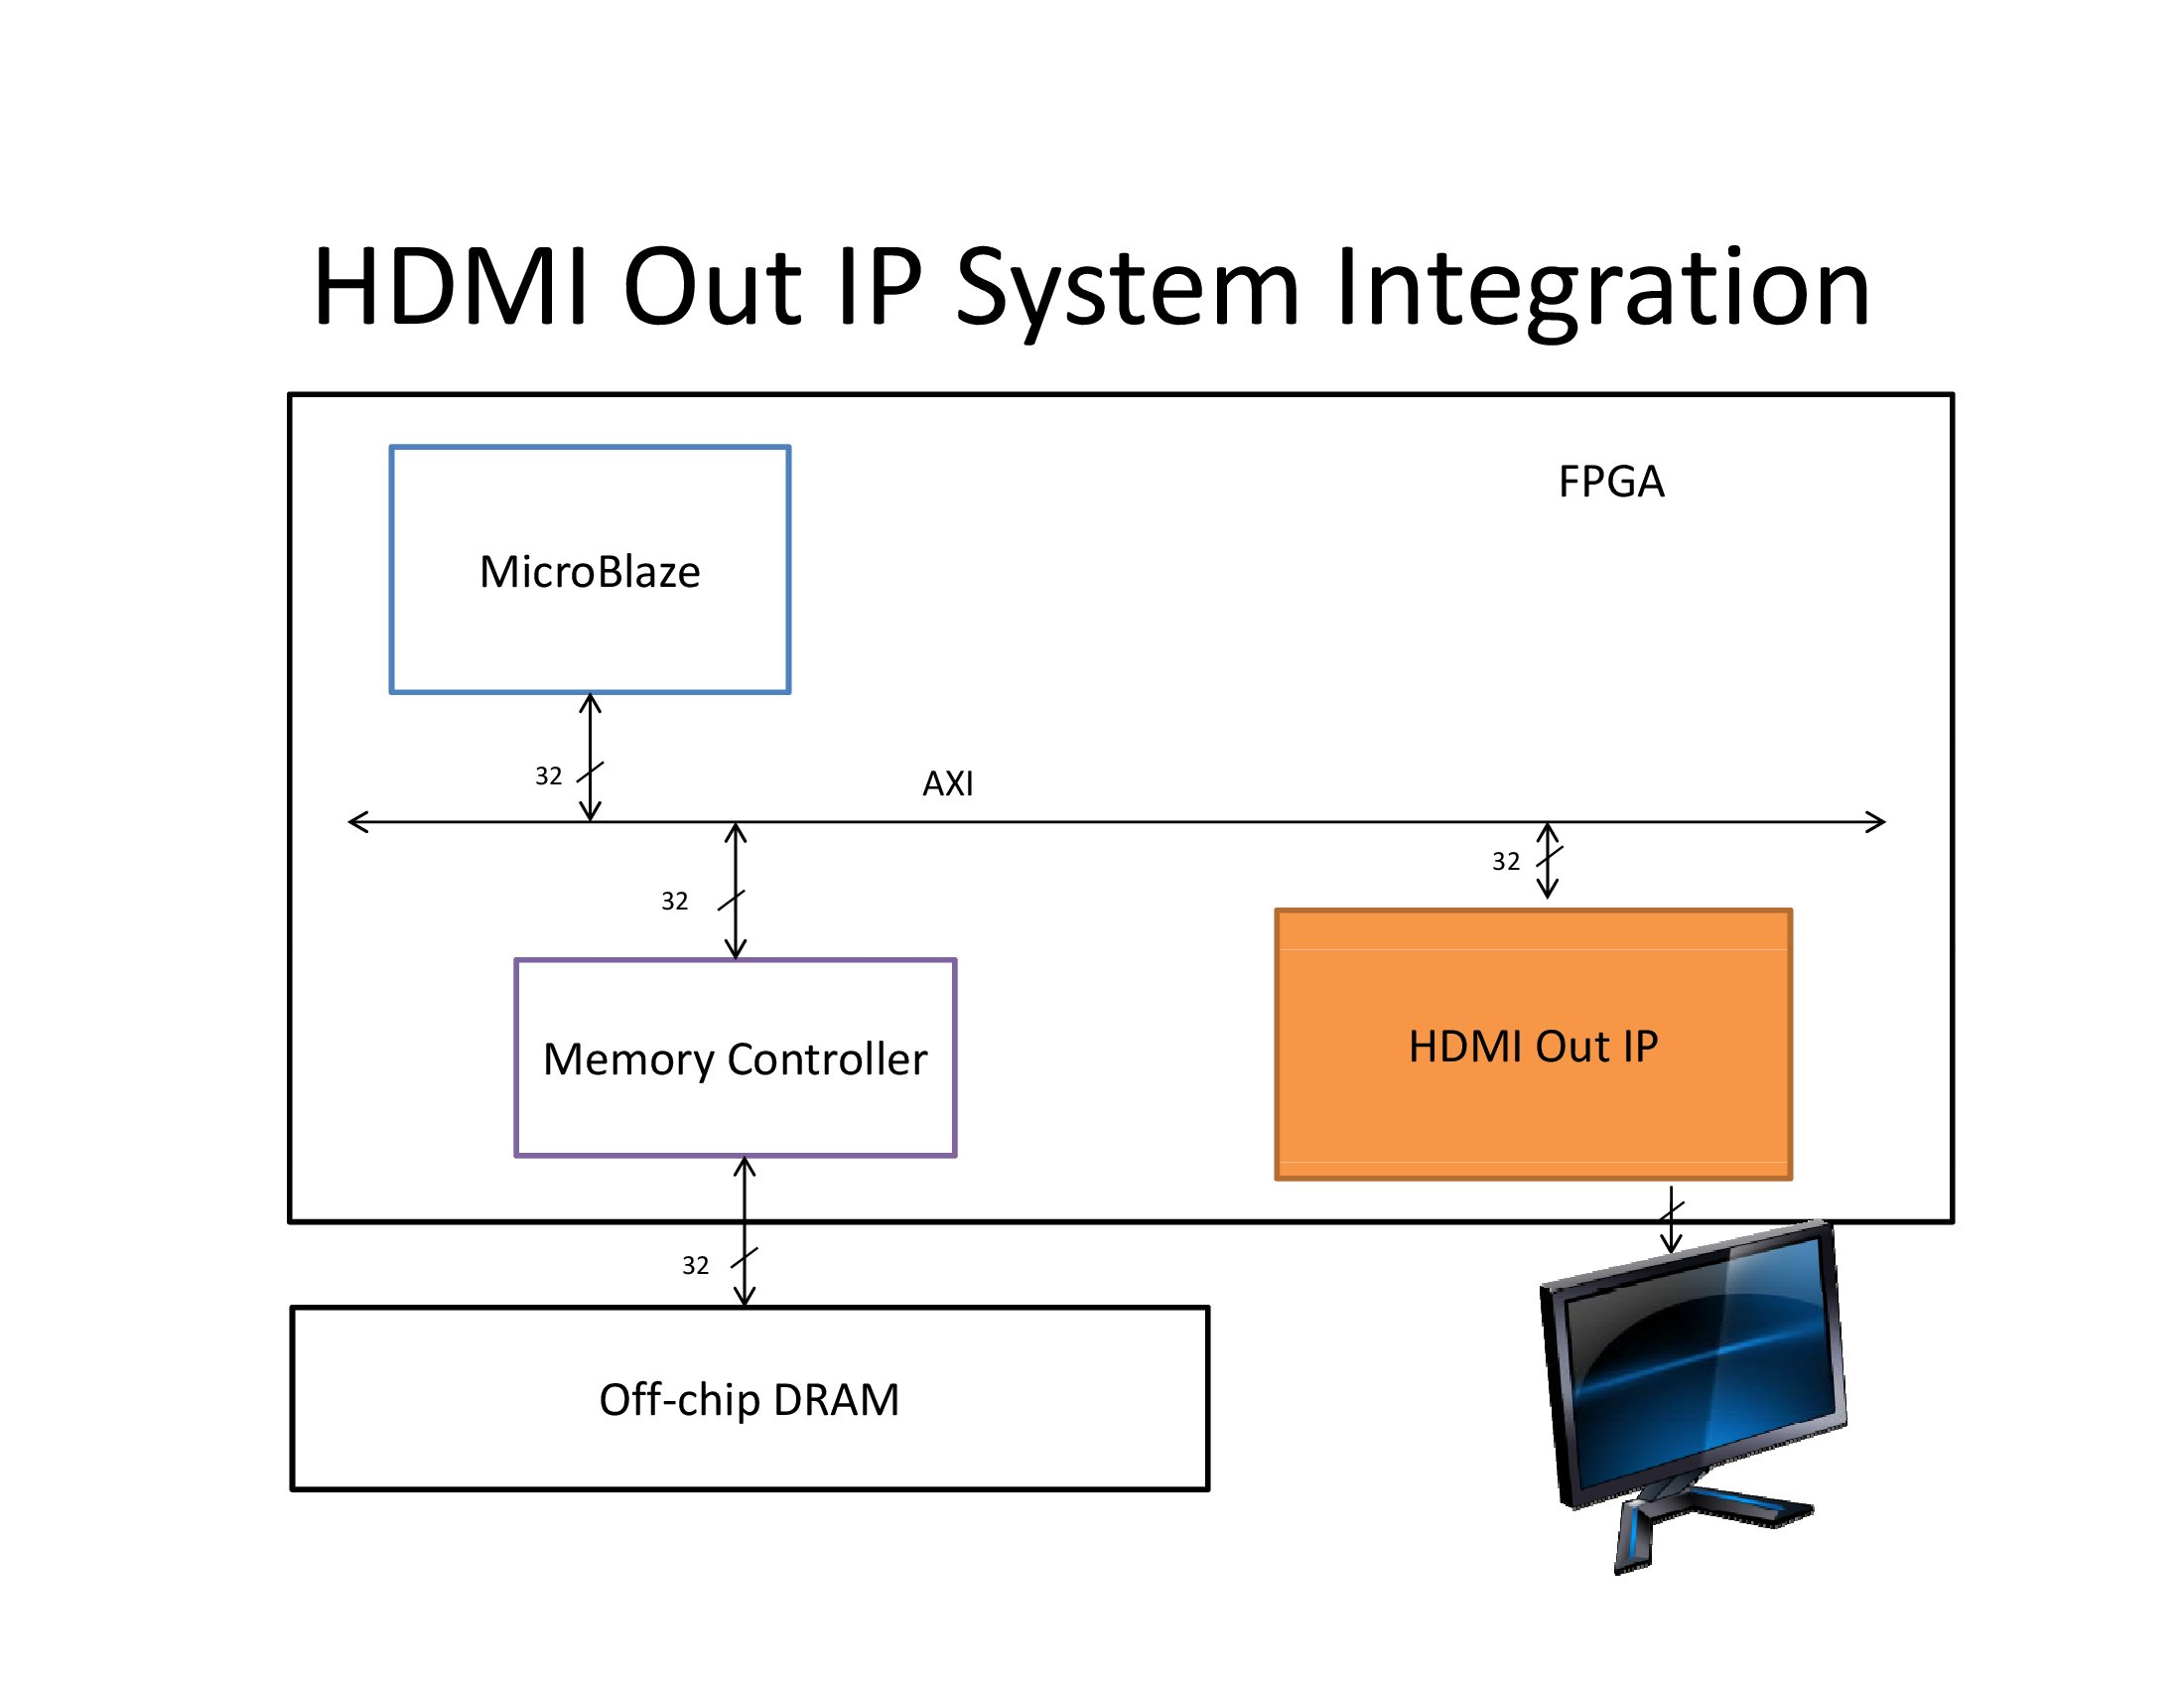
\includegraphics[width=5in] {hdmi_out_fig_system.jpg}}
	\caption{System Integration Block Diagram}
	\end{figure}


	\begin{figure}
	\centering
	\fbox{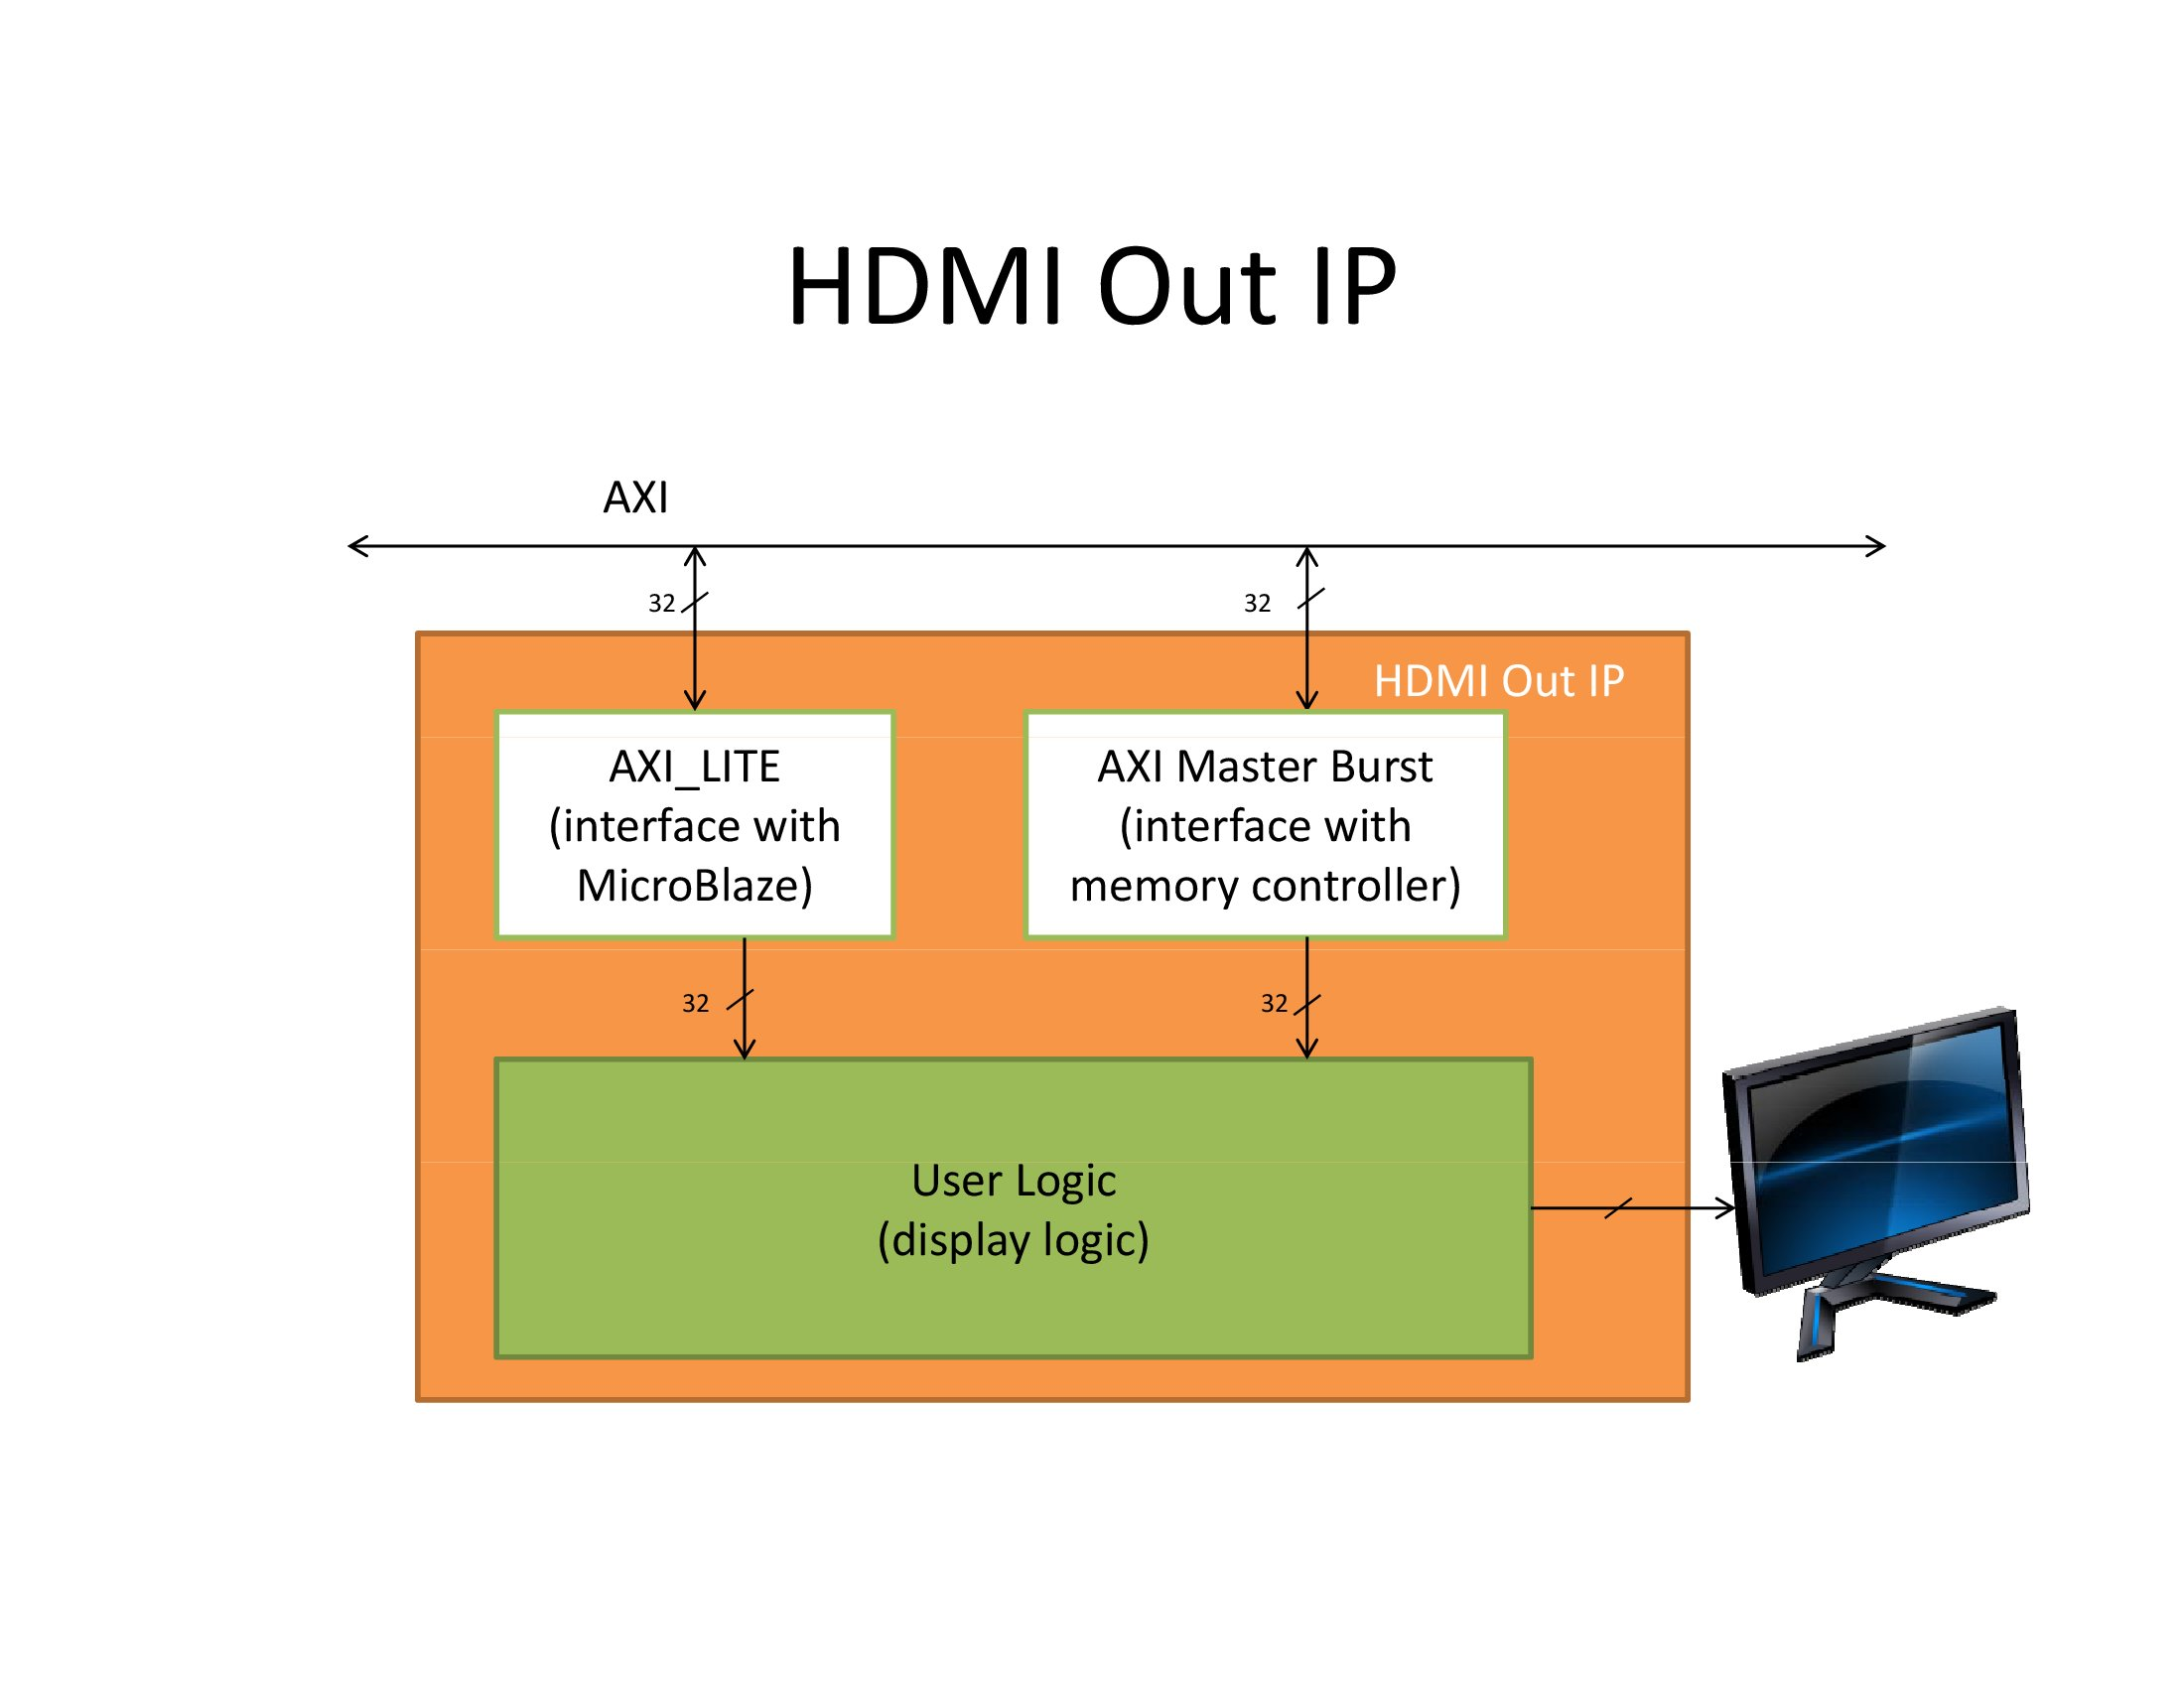
\includegraphics[width=5in] {hdmi_out_fig_ip.jpg}}
	\caption{IP Block Diagram}
	\end{figure}

	\begin{figure}
	\centering
	\fbox{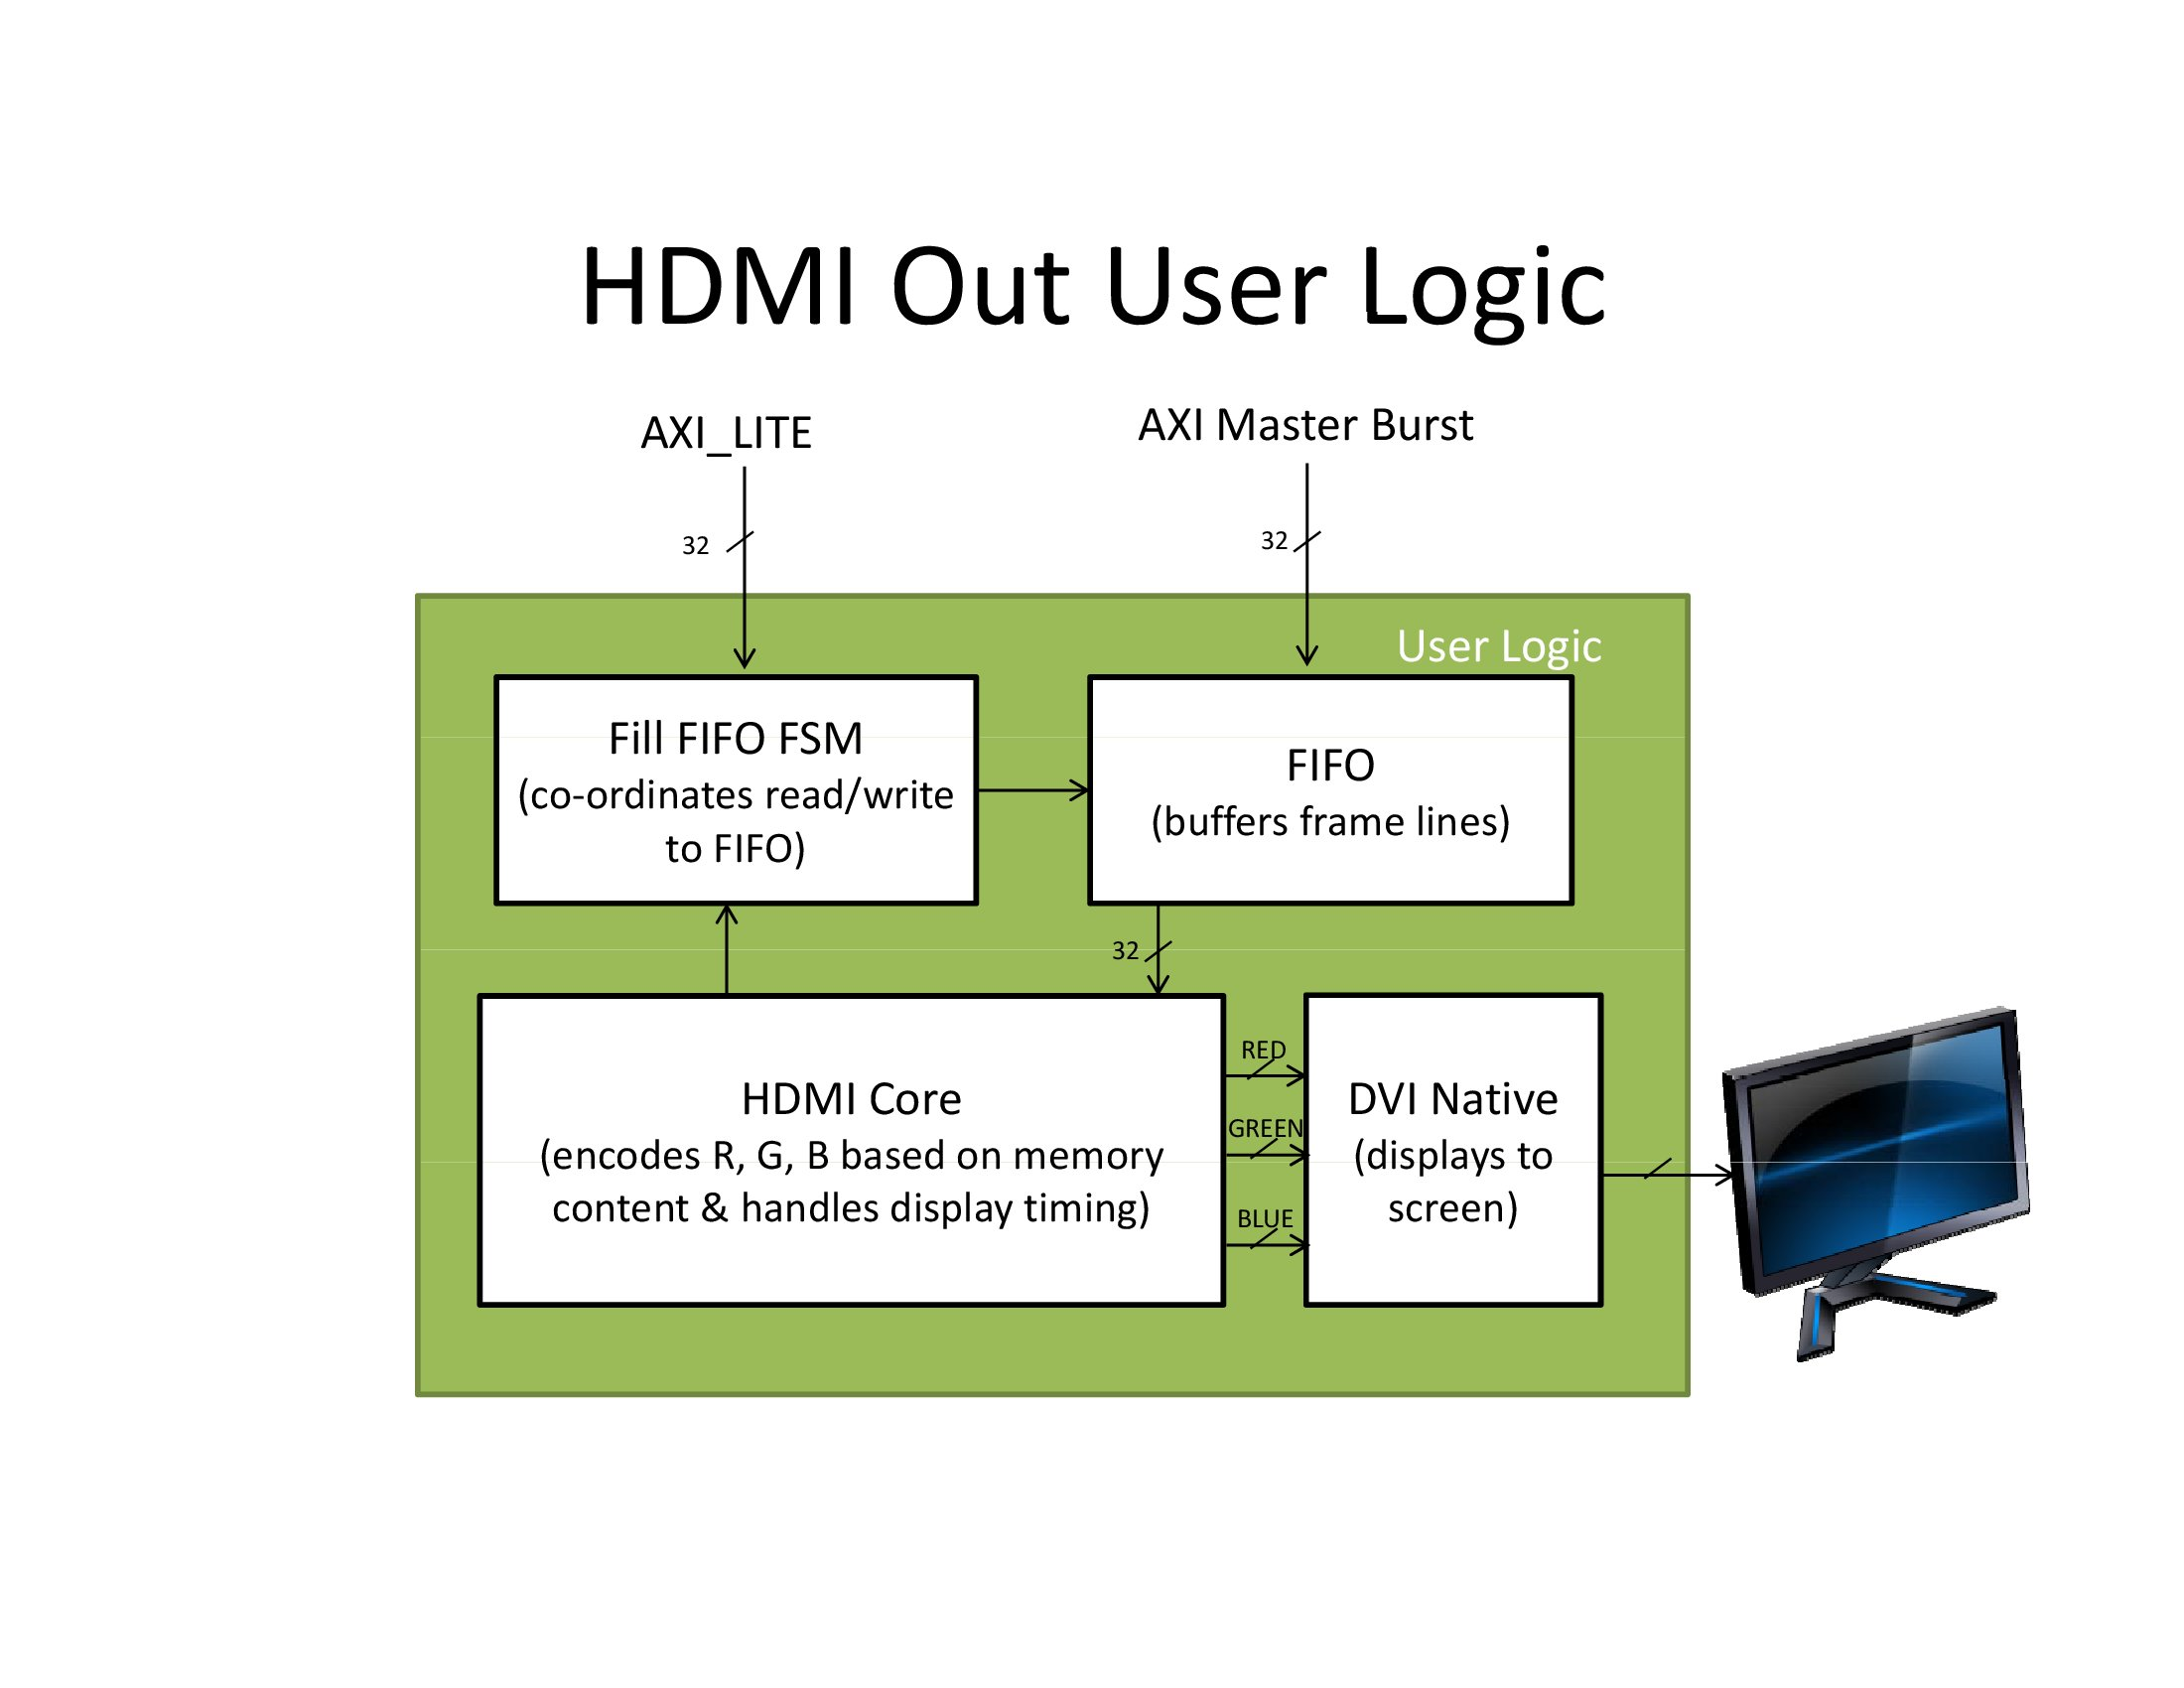
\includegraphics[width=5in] {hdmi_out_fig_userlogic.jpg}}
	\caption{User Logic block diagram}
	\end{figure}
  \section{Setting parameters}
  To change resolution, or to change the colour format, open XPS and change the parameters on the hdmi\_out core. \textbf {HDMI\_HRES} refers to the horizontal resolution. For example, 1280 refers to a resolution of 1280x720. \textbf {HDMI\_NUM\_BYTES\_PER\_PIXEL} refers to the colour format. 2 refers to RGB565 and 4 refers to RGB888x. Note that 640x480 and 800x600 need an input clock of 25MHz, while the 1280x720 resolution needs an input clock of 75MHz. The two projects have the correct clock setup. If you change the parameters, you may also need to change the software. Note that line stride is specified in pixels, so line stride may not need to change if only the colour format is different.
  \section{Software registers}
  \begin{description}
    \item[Software register 0] This is the line stride register. The line stride is measured in \# of pixels.
    \item[Software register 1] This is the address register. Set it to the beginning of the frame you would like to display.
    \item[Software register 2] This is the enable register. Set it to 1 to enable drawing from the specified frame address.
  \end{description}
  See the C code example in \textbf {ip\textbackslash{}workspace\textbackslash{}hdmi\_out\_test\textbackslash{}src\textbackslash{}main.c} for an example on how to set the software registers.
  \section{Caveats}
  Note, the RESET button does not work in resetting the design. The video output will not be stable.
\end{document}
